\documentclass[12pt]{scrartcl}
\usepackage[utf8]{inputenc}
 \usepackage{fancyhdr, graphicx}
 \usepackage[german]{babel}
 \usepackage[scaled=0.92]{helvet}
 \usepackage{enumitem}
 \usepackage{parskip}
 \usepackage{lastpage} % for getting last page number
\usepackage{listings}
\usepackage{caption}
\usepackage{color}
\usepackage{xcolor}
\DeclareCaptionFont{white}{\color{white}}
\DeclareCaptionFormat{listing}{\colorbox{gray}{\parbox{\textwidth}{#1#2#3}}}
\newcommand\Fontvi{\fontsize{6}{7.2}\selectfont}

 \renewcommand{\familydefault}{\sfdefault}
\usepackage[hyphens]{url}
\usepackage[hidelinks]{hyperref}
 
 \fancypagestyle{firststyle}{ %Style of the first page
 \fancyhf{}
 \fancyheadoffset[L]{0.6cm}
 \lhead{
 
\includegraphics[scale=0.8]{./FHNW_HT_10mm.jpg}}
 \renewcommand{\headrulewidth}{0pt}
 \cfoot{Thomas Baumann \& Egemen Kaba}
}

\fancypagestyle{documentstyle}{ %Style of the rest of the document
 \fancyhf{}
 \fancyheadoffset[L]{0.6cm}
\lhead{
 
\includegraphics[scale=0.8]{./FHNW_HT_10mm.jpg}}
 \renewcommand{\headrulewidth}{0pt}
 \lfoot{Laborübung 2}
 \cfoot{Thomas Baumann \& Egemen Kaba}
 \rfoot{\thepage\ / \pageref{LastPage} }
}

\pagestyle{firststyle} %different look of first page
 
\title{ %Titel
Applikationssicherheit 
\vspace{0.2cm}
}

 \begin{document}
 \maketitle
 \thispagestyle{firststyle}
 \pagestyle{firststyle}
 \begin{abstract}
 \begin{center}
 Laborübung 2
 \end{center}
 \vspace{0.5cm}
\hrulefill
\end{abstract}

 \pagestyle{documentstyle}
 \tableofcontents
 \pagebreak
 
\section{Architektur}
Die Architektur ist wie in Abbildung \ref{fig:Arch} implementiert. Dabei haben wir uns an das MVC-Pattern gehalten, damit die Rechte klar getrennt werden.

Sämtliche Anfragen des Client-Browsers werden von einem Servlet entgegengenommen, welches auf einem Tomcat Server läuft. Dieses reicht die Anfragen entsprechend dem page-Parameter und GET bzw. POST die entsprechende Methode des Controllers weiter. Der Controller erstellt, wenn benötigt, ein Objekt der Klasse Company, dem Model, indem er entweder die erhaltenen Daten in eine neu Instanz abfüllt oder mithilfe des CompanyDAO auf die Datenbank zugreift, um von diesem ein Objekt zu erhalten. Über das DAO kann dementsprechend auch ein Company-Objekt gespeichert, bzw. nachgeführt werden. Als Datenbanksystem wird MySQL verwendet. Mit Hilfe des HttpServletRequest werden JavaServer Pages gerendert und als Antwort zurück an den Client gesendet, bzw. über den HttpServletResponse wird eine Weiterleitung ausgelöst.
\begin{figure}
	\centering
	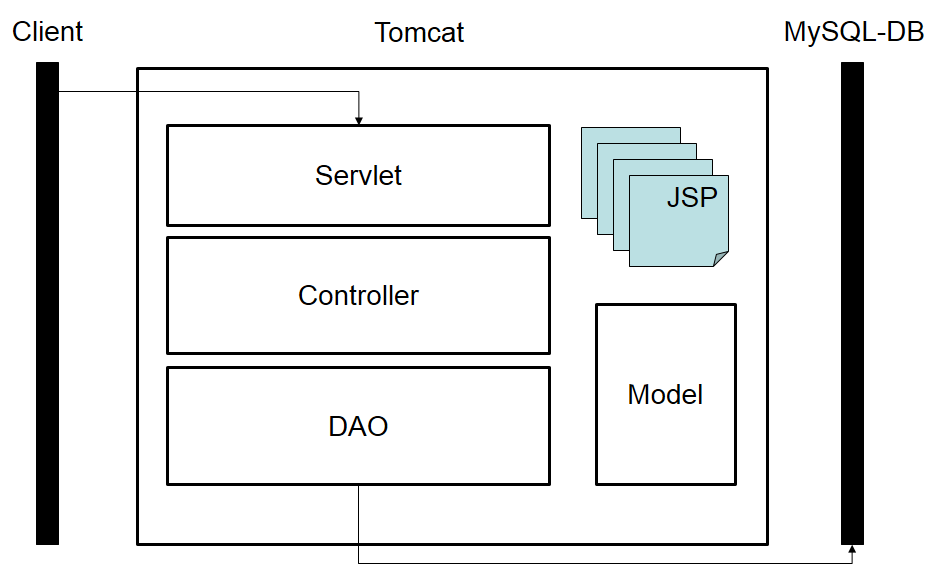
\includegraphics[width=12cm]{./Architektur.png}
	\caption{Architektur}
	\label{fig:Arch}
\end{figure}

\section{Ressourcen}
\textbf{JavaServerPages}\newline
Als View-Schicht werden JavaServerPages verwendet, mit Hilfe deren auch normaler Java-Code ausgeführt werden kann. Der Java Code wird für das anzeigen der Fehler- bzw. Erfolgsmeldungen und der Daten aus der Datenbank / Model verwendet.

Die vom Benutzer eingegebenen Werte in Formularen (POST-Daten) sind implizit in einer Map abgelegt, welche unter dem Namen "param" abrufbar ist. So kann zum Beispiel das Feld "`name"' mit "`\$\{param.name\}"' ausgelesen werden.

Damit die JSP-Seiten nicht direkt aufgerufen werden können, sind sie im WEB-INF Verzeichnis des Tomcat Servers abgelegt.

\textbf{error404.html / error500.html}\\
Eigene Fehlerseiten, die bei Fehlern im Servlet angezeigt werden.

\textbf{config.properties}\\
In dieser Java Property Datei sind die Konfigurationen für das E-Mail-Konto, den Zugriff auf die Datenbank und das Template für die Email abgespeichert. So können diese Einstellungen verändert werden, ohne dass der Code neu kompiliert werden muss.

\textbf{web.xml}\\
Da wir die Servlet Spezifikation Version 3.0 verwenden, kann das Servlet als WebServlet annotiert werden und auch der Security Constraint (Deklaration dass HTTPS verwendet werden muss) kann als Annotation festgelegt werden. Somit muss im Deployment Descriptor bloss das Welcome-File (Startseite) und die Konfiguration der Fehlerseiten definiert werden.

\textbf{database.sql}\\
Mit dieser Datei kann die Datenbank für die Applikation aufgesetzt werden. Dabei werden sowohl die benötigte Datenbank, die Tabelle mit den Spalten, als auch ein Benutzer mit den benötigten Berechtigungen erstellt.

\textbf{https-einrichten.txt}\\
In dieser Datei wird beschrieben, wie https auf einem Tomcat Server aufgesetzt werden kann.

\textbf{build.xml}\\
Das Ant-Script automatisiert das Compilieren, das Erstellen der war-Datei und das Deployment auf den Tomcat Server.

\section{Klassen}
Implementierungsdetails siehe Sourcecode.

\textbf{RattleBitsServlet}\\
Diese Klasse erbt von HttpServlet, ist somit die Schnittstelle der Applikation zur Aussenwelt.\\
In diesem Servlet wird im Konstruktor der Controller sowie die Datenverbindung aufgesetzt. Hier wird ebenfalls auf GET- und POST-Anfragen reagiert und auf den Controller delegiert. Beim Zerstören des Servlets wird die Datenverbindung beendet.

\textbf{Controller}\\
Der Controller verarbeitet Anfragen, die an den Servlet gesendet wurden. Dabei existieren für jede Seite und für jeden Typ einer Anfrage eine entsprechende Methode. Diese prüfen jeweils als erstes, ob der Benutzer bereits eingeloggt ist. Anhand diesem Resultat wird festgestellt, ob der Benutzer die gewünschte Aktion durchführen kann, oder auf eine andere Seite weitergeleitet werden soll.\\
Da diverse Aktionen einen Zugriff auf die Datenbank voraussetzen, wird im Konstruktor ein Data Access Object, das CompanyDAO, mit der übergebenen Connection instanziert.\\
Das Rendern der Seiten, wird über den RequestDispatcher geregelt. Die Strings, welche den Pfad der Views repräsentieren sind dabei als Konstanten definiert.\\
Im Controller wird neben der allgemeinen Koordination ebenfalls das Auslösen der Validierung, des Ladens und Speichern von der Datenbank und das senden der E-Mail vorgenommen.

\textbf{CompanyDAO}\\
Das CompanyDAO ist die Schnittstelle der Applikation zur Datenbank. Im Konstruktor wird deshalb auch eine Connection-Instanz übergeben, in dem Informationen enthalten sind, die für die Verbindung zur Datenbank notwendig sind.\\
Weiter werden einige Methoden bereit gestellt, welche Objekte des Models in der Datenbank persistieren oder mit Informationen aus der Datenbank instanzieren und zurückgeben.\\
Die Abfragen zur Datenbank werden dabei mittels PreparedStatements ausgeführt.

\textbf{Company}\\
Diese Klasse stellt das Model dar. Diese Klasse enthält Informationen, die aus der Datenbank stammen, oder in der Datenbank persistiert werden sollen. Dabei sind alle Felder, die nicht geändert werden sollen als final deklariert und haben dementsprechend auch keinen setter.\\
Sie bietet zudem Methoden an, um die enthaltenen Daten per RegEx zu validieren.

\textbf{MailHelper}\\
Mit Hilfe dieser Klasse kann eine E-Mail versendet werden, dabei wird die Bibliothek javax.mail verwendet. Die Konfiguration für den SMTP-Server und das Template für die Nachricht wird dabei aus der Java Property Datei gelesen.

\textbf{Utility}\\
In der Utility werden zentral statische Methoden angeboten, die an mehreren Stellen in der Applikation verwendet werden. Diese sind im Detail eine Methode zum generieren eines randomisierten Strings gemäss der Passwort-Validations-Methoden sowie eine Methode, um Strings mittels SHA-256 zu hashen. Dabei wird der Hash noch so verändert, dass dieser nur aus Zeichen aus dem Hexadezimalsystem besteht.

\textbf{Verifiers}\\
Die Methoden dieser Klasse, haben die Aufgabe eine PLZ zu verifizieren. Damit die Verifikation nicht auf einen einzelnen Webdienst gestützt ist, wird zuerst versucht auf post.ch zu verifizieren. Schlägt diese Verifikation aufgrund von Verbindungsproblemen fehl, wird die PLZ auf postleitzahlen.ch verifiziert.\\
Bei beiden Varianten kann eine GET-Anfrage gesendet werden, welche mit einer HTML-Seite antworten. Diese wird auf eine Meldung überprüft, welche darauf hindeutet, dass diese PLZ nicht existiert.

\section{Sicherheitsmechanismen}
\subsection{Benutzereingaben}
Die Benutzereingaben werden im Controller aus dem HttpServletRequest geholt und im Model gespeichert. Dieses Model wird dann jeweils immer validiert, bevor etwas weiteres mit den Daten gemacht wird. Die Validation findet dabei mithilfe von Regulären Ausdrücken statt. Wenn die Daten nicht korrekt sind werden sie nicht weiterverwendet und eine Fehlermeldung an den Client gesendet.\\
Da gemäss Aufgabenstellung keine Sicherheitskritische Zeichen zugelassen sind, müssen diese auch nicht bearbeitet werden. Wenn solche (z.B. $'$ oder $<$) gültig wären, müssten diese noch ersetzt bzw. escaped werden.\\
Damit an der Datenbank keine SQL-Injection Angriffe vorgenommen werden können, werden die validen Benutzereingaben mit Hilfe von PreparedStatements verarbeitet.\\
Um die Benutzerfreundlichkeit zu unterstützen, werden alle Benutzereingaben bei Fehlermeldungen wieder angezeigt. Damit ein Benutzer auf sich selber keine XSS-Attacke ausführen kann, bzw. die Seite nicht falsch dargestellt wird. Werden die Benutzereingaben mit Hilfe der JavaServer Pages Standard Tag Library ($jstl/core:out$) bearbeitet. Dabei werden verbotene Zeichen durch die entsprechenden HTML-Zeichen ersetzt.\\
Beim Anzeigen von Daten aus der Datenbank werden keine Vorkehrungen getroffen, da davon ausgegangen wird, dass nur sichere Daten, welche unsere gespeicherten Daten sind, in der Datenbank abgelegt werden.

\subsection{E-Mail}
Die E-Mail-Validierung wird durch die Klasse EmailValidator der Apache Commons Bibliothek gelöst. Diese überprüft dabei nur, ob die E-Mail Adresse syntaktisch korrekt ist.\\
In unserer Lösung ist die E-Mail-Verifizierung nicht implementiert, da es keine 100\%ige Möglichkeit gibt im Voraus zu bestimmen, ob eine E-Mail Adresse existiert. Eine Möglichkeit wäre die "`Callback verification"' (\url{http://en.wikipedia.org/wiki/Callback_verification}), dabei wird eine Anfrage an den Mailserver gesendet und dieser sollte eine Antwort zurückgeben, ob die Adresse existiert. Die ist jedoch bei vielen Mailservern deaktiviert, damit dies nicht für SPAM-Mail missbraucht werden kann. Die zweite Möglichkeit wäre den SMTP-Befehl "`$VRFY$"' an den Mailserver zusenden, welcher genau für diesen Zweck gedacht wäre, aber auch dieser ist bei vielen Servern deaktiviert.\\
Das Versenden von E-Mails wird schlussendlich durch den MailHelper übernommen, welcher intern javax.mail verwendet.

\subsection{PLZ}
Die PLZ-Validierung wird wie die restlichen Benutzereingaben per Regulären Ausdruck validiert.\\
Die PLZ-Verifizierung erfolgt durch einen von zwei Webdienste. Der erste Webdienst der angesteuert wird, ist derjenige von post.ch. Gibt es bei der Verbindung zu diesem Webdienst ein Problem, wird auf den Webdienst von postleitzahlen.ch zurückgegriffen. Bei beiden Varianten können eine GET-Anfrage durchgeführt werden, da die PLZ vorgängig per Regulären Ausdruck validiert wurde enthält sie genau 4 Zahlen und kann somit direkt übergeben werden. Die Antwort wird anschliessend auf ein Stichwort untersucht, welches indiziert, dass die PLZ nicht gefunden wurde. Durch die zwei Webdienst wird sichergestellt, dass die Verfügbarkeit möglichst auf einem hohen Level gehalten werden kann.\\
Eine optimalere Lösung, jedoch nicht gemäss Aufgabenstellung, wäre alle PLZ lokal in einer Datenbank zu speichern. Somit müsste nicht jedes mal eine weitere Webseite aufgerufen werden, welche eine zusätzliche Verzögerung verursacht. Diese Datenbank müsste etwa jährlich mit den neuesten Daten befüllt werden,

\subsection{HTTPS}
Damit ein Tomcat Server HTTPS unterstütz, muss dieser zuerst konfiguriert werden, dabei müssen zwei Schritte vorgenommen werden:
\begin{itemize}
	\item Generieren eines Keystores mittels keytool von Java
	\item Konfigurationsdatei des Tomcat Servers anpassen, dass er den Keystore findet und öffnen kann
\end{itemize}
Eine detaillierte Beschreibung ist in der Datei rsc/https-einrichten.txt der Applikation zu finden.

Damit der Tomcat Server automatisch eine HTTPS-Verbindung verwendet (SecurityConstraint), muss dies im Deployment Descriptor (web.xml) definiert werden, oder das Servlet kann mit $@ServletSecurity$ annotiert werden, was in unserem Fall gemacht wurde. Damit müssen alle Verbindungen zu unserem Servlet über HTTPS laufen, sollte eine Anfrage über die ungesicherte Leitung HTTP kommen, so wird diese automatisch umgeleitet.\\
Da wir ein einziges Servlet implementiert haben, ist es mit dieser Lösung nicht möglich nur bestimmte Seiten über HTTPS laufen zu lassen. (Es kann kein URL-Mapping auf ein Query vorgenommen werden.) Diese Lösung hat aber den Vorteil, dass sämtliche Kommunikation mit der Applikation über HTTPS erfolgt, was die Sicherheit erhöht.\\
Eine andere Lösungsmöglichkeit wäre gewesen, einen Filter zu implementieren, der bei jeder Anfrage aufgerufen wird. Dieser müsste jedesmal kontrollieren, welche Seite aufgerufen wurde und ob sie, wenn benötigt über HTTPS aufgerufen wurde. In diesem Fall darf kein SecurityConstraint definiert sein und der Programmierer muss selber schauen, dass wirklich HTTPS verwendet wird.\\
Eine weitere Möglichkeit wäre für jede Seite ein eigenes Servlet zu erstellen und für jedes einen SecurityConstraint zu definieren. Damit kann für jede Seite einzeln entschieden werden, ob sie über HTTPS laufen muss oder nicht.

\subsection{Bedrohungsmodell Datenbank}
Für die Applikation wurde ein neuer Benutzer erstellt, welcher nur $SELECT$, $INSERT$, $UPDATE$ und $DELETE$ auf der eigens dafür erstellten Datenbank durchführen kann (siehe rsc/database.sql). Somit ist es unmöglich auf andere Datenbanken zuzugreifen, oder eine Tabellenstruktur zu bearbeiten.\\
Weiter sollte das Datenbanksystem so konfiguriert werden, dass nur vom lokalen System zugegriffen werden kann. Somit ist es unmöglich von einem entfernten Computer direkt auf das Datenbanksystem zuzugreifen. Sollte der Webserver auf einem anderem Rechner laufen, so sollte nur für genau diesen Computer eine Berechtigung gegeben werden.\\
Eine weitere Bedrohung stellt SQL-Injection dar. Dies wird jedoch durch die Sicherheitsmechanismen, die im Kapitel über Benutzereingaben beschrieben werden, verunmöglicht.

\subsection{Strategie Login-Versuche}
Unsere Strategie für mehrmalige falsche Login-Versuche umfasst zwei zusätzliche Spalten in der companies Tabelle. Die erste Spalte enthält die Anzahl Fehlversuche seit dem letzten login und die zweite Spalte enthält einen optionalen Zeitstempel, welcher anzeigt, bis wann die Benutzeranmeldung gesperrt ist.\\
Meldet sich ein Benutzer erfolgreich an, so wird der Zähler auf null gesetzt und der Zeitstempel gelöscht. Findet ein Fehlversuch statt, so wird der Zähler um eins erhöht und ab einem Wert von beispielsweise drei, wird ein Zeitstempel gesetzt, der eine Minute in der Zukunft liegt. Somit ist es während der nächsten Minute nicht möglich sich anzumelden und der Benutzer bekommt dementsprechend eine Nachricht.

\subsection{Login und Identifikation}
Der Benutzername wird aus dem Firmennamen und einer angehängten Zahl generiert. Die erste Firma erhält dabei als Zahl die eins. Eine zweite Firma mit dem \textbf{gleichen} Namen erhält den Zusatz zwei. Beim generieren der Zahl, wird jedesmal in der Datenbank kontrolliert, ob der Benutzername bereits existiert.\\
Das Passwort ist ein randomisierter String, welches zuerst per SHA-256 gehasht und dann in Zeichen aus dem Hexadezimalsystem konvertiert wird. Die Konvertierung erhöht die Sicherheit der gespeicherten Passwörter nochmals, falls ein Angreifer zugriff auf die verschlüsselten Passwörter hat und diese knacken will. Der Benutzer erhält den randomisierten String per E-Mail zugesendet. In der Datenbank wird das gehashte und konvertierte Passwort gespeichert.\\
Wenn sich ein Benutzer anmeldet, so wird der Benutzer mit dem angefordertem Benutzernamen aus der Datenbank ausgelesen und erst im Controller, also im Java-Code, wird das übereinstimmen des Passwortes überprüft. Dies ist eine weitere Sicherheitsmassnahme gegen eine SQL-Injection. Bei erfolgreichem Login, erhält der User eine Id zugewiesen. Diese entspricht der Id in der Datenbank, welche bei der Registrierung einer Firma angelegt wird (Primarykey mit autoincrement). Zusätzlich wird dem User ein randomisierter String, mit der Länge von 64 Zeichen (a-z, A-Z, 0-9), zugewiesen, welcher bei jedem Login neu generiert wird und in der Datenbank gespeichert wird. Beide Informationen werden in der Session des Nutzers gespeichert. Loggt sich der Benutzer aus, so werden die Session Daten und der String in der Datenbank gelöscht.\\
Mit diesen Informationen kann festgestellt werden, ob der Nutzer eingeloggt ist und ob dieser Nutzer, Informationen in der Session manipuliert hat. Denn ist die Kombination aus Id und String nicht in der Datenbank vorhanden, wird dem Nutzer die Zugriff auf weitere Seiten innerhalb des geschützten Bereichs verweigert.

\subsection{Interne Fehler}
Treten jegliche Fehler innerhalb des Servlets auf, werden diese nicht die original Fehlermeldungen mit dem Stacktrace an den Benutzer weitergeleitet, sondern eigene definierte Fehlermeldungen angezeigt.\\
Ein Mapping im Deployment Descriptor verweist je nach Fehlermeldung auf eine andere Fehlerseite. Dabei unterscheiden wir zwischen einem 404 Fehler und allen anderen Fehler, die wir als 500 Fehler darstellen. Diese Massnahme wurde getroffen, damit der Benutzer keine Informationen über das System erhalten kann und somit einem Angreifer helfen würde.

\subsection{viele Benutzer}
Da die Applikation stateless ist, die einzigen Zustände welche gespeichert werden, ist die Datenbankverbindung und die Informationen einer Firma, können eine beliebige Anzahl Benutzer auf das Servlet zugreifen. Da Referenzen auf company-Objekte nur lokal in einer Methode vorhanden sind, können sich mehrere Threads nicht in die quere kommen. Das einzige Problem wäre die Verifizierung der PLZ über einen Webdienst. Dies sollte aus Performance gründen in diesem Fall zwingend mit Hilfe einer lokalen Datenbank vorgenommen werden.

\end{document}